\chapter {Produktfunktionen}

\subsection{Grundfunktionalität}
\setcounter{counterKriterien}{0}
%\subsubsection{Graphische Bedienoberfläche}

\nItem{PF} Startbildschirm \\
Nach dem Start der Anwendung werden dem Benutzer die zuletzt geöffneten Projekte angezeigt. Der Benutzer
hat dann die Möglichkeit ein bereits bestehendes Projekt zu öffnen oder ein neues anzulegen.
 
% Es ist unsinnig zwischen Filtern und Testsignalen zu unterscheiden. Wie soll ein Testsignal aussehen ?
\nItem{PF} Filtercontainer \\
Der Filtercontainer ist die Stelle der grafischen Oberfläche, an der der Nutzer einen der Anwendung
zur Verfügung stehenden Filter auswählen kann (durch einen Klick mit der Maus). Um einen Filter auszuwählen
muss ein gültiges Video im Projektexplorer gewählt worden sein. Durch die Auswahl eines Filters wird
der entsprechende Filter als der nächste anzuwendende Filter markiert. Dem Benutzer steht die Möglichkeit offen, einen bereits gewählten Filter wieder abzuwählen.
% Man sollte wahrscheinlich erwähnen, dass es nicht möglich sein wird das Video abzuspielen bis der Filter 
% tatsächlich angewandt wurde.

%  Wieder eine in meinen Augen nicht zielführende Unterscheidung zwischen Typen von Videos. 
%  Eine vlcht. geschicktere Version:
\nItem{PF} Projektexplorer \\
Nachdem ein bestehendes Projekt geöffnet oder ein neues erstellt worden ist wird dem
Benutzer unter anderem ein Projektexplorer zur Verfügung gestellt. Ein Projektexplorer ist ein 
Fenster das zwei Registerreiter enthält. \\
Der erste Reiter, die \emph{SmartTree}, enthält dem Projekt zugewiesene Videosequenzen. Dabei wird
grundsätzlich zwischen Referenz- und erzeugten Sequenzen unterschieden. Wie in Abb.\ref{pExplorer}
ersichtlich, hat die SmartTree eine Baumstruktur, dabei ist jedes Vaterelement
ein Referenzvideo im Bezug zu seinen Kindelementen. Beispielsweise ist in Abb.\ref{pExplorer}
">Carphone.yuv"< ein Referenzvideo im Bezug zum Kindelement ">Gaussian Blurr"<. Gaussian Blurr ist ein
vom Nutzer gewählter Name für die Videosequenz ">Carphone.yuv"< an der der gaußsche Weichzeichner angewandt
wurde und ">processed"< ist der vom Nutzer gewählter Name für die ">Gaussian Blurr"< Videosequenz auf
der er sein \gls{glos:VBW} ausgeführt hat. Jedes der in der \emph{SmartTree} aufgeführten Videos wird im Projektordner oder in einem vom Benutzer angegebenen Stelle seiner Festplatte abgelegt.\\
Der zweite Reiter \emph{Dateiexplorer} stellt eine Schnittstelle zum Dateisystem des Benutzers dar. Mit Hilfe
des Dateiexplorers kann der Nutzer \projektTitel neue Videosequenzen bekannt machen.
\begin{figure}[h]
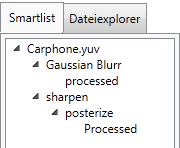
\includegraphics[scale=1]{bilder/projektexplorer.png}
\caption{Projektexplorer}
\label{pExplorer}
\end{figure}

\nItem{PF} Filtervorgang\\
Nachdem der Nutzer einen oder mehrere Filter gemäß der PF Filtercontainer markiert hat, kann er
den Filtervorgang durch den Klick auf das entsprechende Symbol in der Toolbar oder im Hauptmenü
einleiten. Die Dauer des Filtervorgangs ist abhängig von der Anzahl der gewählten Filter und der Auflösung
und Länge des gewählten Videos. Nach einem Filtervorgang wird das neu entstandene Video
als Kindelement des für den Filtervorgang ausgewähltem Videos aufgeführt.\\
\nItem{PF} Graphische Oberfläche \\
\gls{OQAT} stellt dem Nutzer eine Interaktive Benutzeroberfläche zur Verfügung, die
einzelnen Bestandteile dieser werden im Kapitel \emph{Graphische Oberfläche} näher erläutert.\\
% Gleiches Argument wie oben, das Zeug ist noch nicht sortiert. Da sind pseudoKapitel nur verwirrend.
%\subsubsection{Projektverwaltung}
% Etwas ungenau, sowas haben wir bereits in dem MK. An dieser Stelle muss man also etwas spezifiescher
% werden
\nItem{PF} Projekte anlegen \\
Um \gls{OQAT} verwenden zu können, muss der Benutzer ein neues Projekt anlegen oder
ein bereits existierendes öffnen. \\
Ein neues Projekt kann entweder über das Hauptmenü, die Toolbar oder mit Hilfe des sich
im Startfenster befindenden Buttons angelegt werden. Nachdem der Nutzer eine dieser Möglichkeiten
in Anspruch genommen hat, öffnet sich Projekterstellungs-Dialog. In diesem Dialog
muss der Benutzer folgende Daten angeben:
\begin{compactitem}
\item Projektname
\item Ein Pfad unter dem die Projektdaten abgelegt werden sollen. Dieses kann auch leer gelassen werden, 
dann wird ein Defaultpfad verwendet.
\end{compactitem}

%\subsubsection{Portabilität}
%
%\subsubsection{Analyse}
\nItem{PF} MetriList\\
Die \emph{MetriList} enthält alle der Anwendung zur Verfügung stehenden Analysemetriken.
Sobald im SmartTree ein Video und ein gültiges Referenzvideo ausgewählt wurde, kann der Benutzer
eine oder mehrere Metriken auswählen. Eine erfolgreiche Auswahl wird durch das hervorheben des
jeweiligen Eintrags der \emph{MetriList} und einen entsprechenden Vermerk in dem Visualisierungsbereich
gekennzeichnet. Eine Metrik kann erst ausgewählt werden, wenn möglicherweise zuvor gewählte Filter
z.B. durch den Klick auf das entsprechende Symbol der Toolbar bereits angewandt wurden. Versucht
der Benutzer eine Metrik auszuwählen ohne ein Video und Referenzvideo entsprechend markiert zu haben oder
während markierte aber nicht abgearbeitete Filter existieren wird er darauf hingewiesen.\\
\nItem{PF} Analysevorgang \\
Nachdem der Nutzer eine oder mehrere Metriken aus der \emph{MetriList} und ein
Video samt einem Referenzvideo ausgewählt hat, kann der Benutzer einen Analysevorgang starten. Hat der
Nutzer mehrere Metriken ausgewählt werden diese im Batchverfahren abgearbeitet. Nachdem ein Analysevorgang
beendet wurde, stehen dem Nutzer die Ergebnisse im Visualisierungsbereich zur Verfügung (wurden 
mehrere Metriken angewandt, so werden diese unter verschiedenen Registerreitern des Visualisierungsbereichs
abgelegt). Die Art der Darstellung der Analyseergebnisse hängt ganz und gar von der Art der gewählten 
Metrik ab. Wenn Beispielsweise die Metrik \gls{mse} gewählt wurde, wird neben dem Differenzvideo, in dem jedes Pixel den jeweiligen \gls{mse} Wert dieser Stelle trägt, auch der globale \gls{mse} für das jeweilige Frame und für die gesamte Videosequenz dargestellt.

\subsection{Optionale Funktionalität}
\setcounter{counterKriterien}{0}
\nItem{OF} Motion Vektoren des .H264 Encoders des \gls{ITEC}\\
Der .H264 Encoder des Instituts liefert, neben der encodierten Videosequenz, auch die verwendeten Motion
Vektoren in einem Datensatz. \gls{OQAT} kann diese Vektoren im Visualisierungsbereich darstellen.\\
\nItem{OF} Drag and Drop\\
Der Projektexplorer ist \emph{Drag and Drop} fähig, d.h. eine gültige Videodatei kann nicht nur über
die Toolbar oder das Hauptmenü hinzugefügt werden, sondern darf auch nach dem \emph{Drag and Drop} Prinzip
in die SmartTree eingefügt werden. Das einzubindende Video kann dabei als ein neues Element (ohne
Vaterelement) oder aber als Kindelement eines bereits vorhandenen Videos eingefügt werden.
